\documentclass[tikz]{standalone}

\usepackage{tikz}
\usetikzlibrary{positioning,trees,decorations.pathreplacing}

\begin{document}
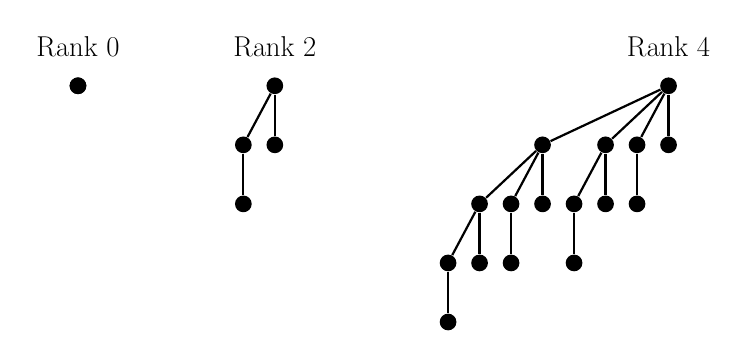
\begin{tikzpicture}[thick,scale=0.5, every node/.style={scale=0.5},grow via three points={%
one child at (0,-1.5) and 
two children at (0,-1.5) and (-0.8,-1.5) 
}
]
    \tikzstyle{marrs}=[very thick,-latex]
    \tikzstyle{tnode}=[circle, fill=black, inner sep=1.5mm]
    \def\rstep{5cm}
    
    \huge
    
    \node[tnode] (0, 0) {};
            child { node[tnode] {} }
            child { node[tnode] {} };
    
    \begin{scope}
        \draw (0, 1) node {Rank 0};
        \node[tnode] (0, 0) {};
    \end{scope}
        
    \begin{scope}[xshift=1 * \rstep]
        \draw (0, 1) node {Rank 2};
        \node[tnode] {}
            child {node[tnode] {} }
            child {node[tnode] {} 
                    child {node[tnode] {} }};
    \end{scope}
    
    \begin{scope}[xshift=3 * \rstep]
      \draw (0, 1) node {Rank 4};
      \node[tnode] {}
          child {node[tnode] {} }
          child {node[tnode] {} 
            child {node[tnode] {} }
          }
          child {node[tnode] {} 
            child {node[tnode] {} }
            child {node[tnode] {} 
              child {node[tnode] {} }
            }
          }
        child[missing] {}
        child {node[tnode] {}
          child {node[tnode] {} }
          child {node[tnode] {} 
            child {node[tnode] {} }
          }
          child {node[tnode] {} 
            child {node[tnode] {} }
            child {node[tnode] {} 
              child {node[tnode] {} }
            }
          }
     };
      \end{scope}
\end{tikzpicture}
\end{document}

